\documentclass[crop,tikz]{standalone}

\usepackage{pgfplots}
\pgfplotsset{compat=1.16}

\begin{document}
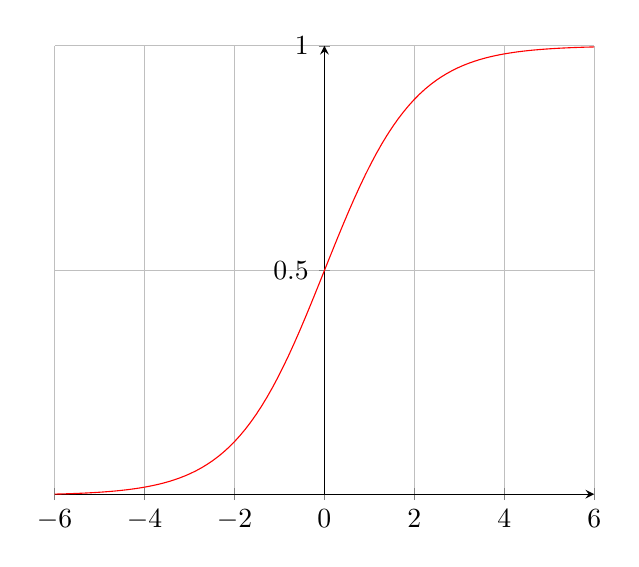
\begin{tikzpicture}[declare function={sigma(\x)=1/(1+exp(-\x));}]
  \begin{axis}
    [
      grid=major,     
      xmin=-6,
      xmax=6,
      axis x line=bottom,
      ytick={0,.5,1},
      ymax=1,
      axis y line=middle,
      samples=100,
      domain=-6:6
    ]
      \addplot[red, mark=none] (x,{sigma(x)});
    \end{axis}
  \end{tikzpicture}
\end{document}
